%%
%% GAC Advisor Presentation
%% When Smaller Is Slower: Dimensional Collapse in Compressed LLMs
%%
\documentclass[aspectratio=169,10pt]{beamer}

\usetheme{metropolis}
\usepackage{booktabs}
\usepackage{graphicx}
\usepackage{tikz}
\usetikzlibrary{positioning,decorations.pathreplacing,fit,backgrounds}
\usepackage{amsmath}
\usepackage{xcolor}
\usepackage{colortbl}

%% Custom colors
\definecolor{cblue}{RGB}{55,131,187}
\definecolor{cred}{RGB}{211,63,73}
\definecolor{cgreen}{RGB}{56,158,92}
\definecolor{corange}{RGB}{230,159,0}

\setbeamercolor{frametitle}{bg=cblue!90!black}
\setbeamercolor{progress bar}{fg=cblue}

\title{When Smaller Is Slower}
\subtitle{Dimensional Collapse in Compressed LLMs}
\author{Jihao Xin}
\institute{KAUST}
\date{February 2026}

\begin{document}

% ============================================================
{
\setbeamertemplate{footline}{}
\begin{frame}
\titlepage
\end{frame}
}

% ============================================================
\begin{frame}{Outline}
\tableofcontents
\end{frame}

% ============================================================
\section{Problem \& Motivation}
% ============================================================

\begin{frame}{Why Compress LLMs?}

\textbf{Large Language Models are expensive to deploy.}

\vspace{0.4cm}
\begin{columns}
\begin{column}{0.5\textwidth}
\begin{tabular}{lr}
\toprule
\textbf{Model} & \textbf{Params} \\
\midrule
Llama-3-8B & 8B \\
Llama-3-70B & 70B \\
Llama-3-405B & 405B \\
\bottomrule
\end{tabular}

\vspace{0.4cm}
\textbf{Key bottleneck}: Memory bandwidth.\\[0.2cm]
Decode is memory-bound --- smaller weights $\Rightarrow$ faster token generation.
\end{column}
\begin{column}{0.5\textwidth}
\textbf{Post-training compression}:\\[0.2cm]
\begin{itemize}
\item No retraining needed
\item Apply to any pre-trained model
\item Reduce memory footprint
\item Should reduce latency\ldots
\end{itemize}

\vspace{0.3cm}
\textbf{Common methods}:
\begin{itemize}
\item Quantization
\item Sparsification
\item \textbf{Low-Dimensional Compression}
\end{itemize}
\end{column}
\end{columns}
\end{frame}

% ------------------------------------------------------------
\begin{frame}{Compression Changes Tensor Dimensions}

\textbf{Key insight}: Many compression techniques alter the \emph{shape} of tensors.

\vspace{0.3cm}
\begin{center}
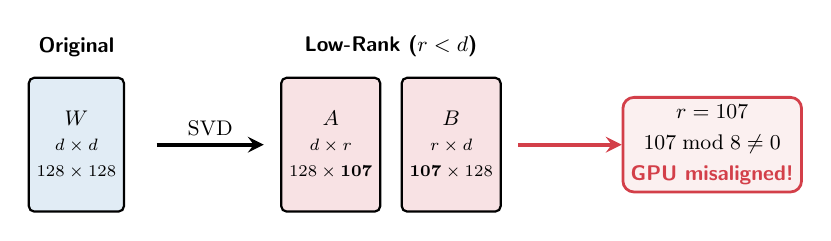
\begin{tikzpicture}[scale=0.85, every node/.style={scale=0.85},
    >=stealth,
    mat/.style={draw, minimum width=1.2cm, minimum height=2.0cm, line width=0.8pt,
                font=\sffamily\small, align=center, rounded corners=2pt}
  ]
  % Original
  \node[mat, fill=cblue!15] (W) at (0,0) {$W$\\{\scriptsize $d \times d$}\\{\scriptsize $128 \times 128$}};
  \node[above=0.15cm of W, font=\sffamily\bfseries\small] {Original};

  % SVD arrow
  \draw[->, line width=1.5pt] (1.2,0) -- (2.8,0) node[midway, above, font=\small] {SVD};

  % SVD result
  \node[mat, fill=cred!15] (A) at (3.8,0) {$A$\\{\scriptsize $d \times r$}\\{\scriptsize $128 \times \mathbf{107}$}};
  \node[mat, fill=cred!15] (B) at (5.6,0) {$B$\\{\scriptsize $r \times d$}\\{\scriptsize $\mathbf{107} \times 128$}};
  \node[above=0.15cm of A, font=\sffamily\bfseries\small, xshift=0.9cm] {Low-Rank ($r < d$)};

  % The problem
  \node[draw, rounded corners=4pt, fill=cred!8, draw=cred, line width=1pt,
        font=\sffamily\small, align=center] (problem) at (9.5, 0) {
    $r = 107$\\[2pt]
    $107 \bmod 8 \neq 0$\\[2pt]
    \textcolor{cred}{\textbf{GPU misaligned!}}
  };
  \draw[->, line width=1.5pt, cred] (6.6,0) -- (problem.west);
\end{tikzpicture}
\end{center}

\vspace{0.2cm}
\textbf{Rank $r$ is determined by importance scoring} (Fisher, magnitude, activation, gradient).

These scores are continuous-valued $\Rightarrow$ after budget allocation, ranks are \textbf{naturally irregular}.

\vspace{0.3cm}
\small
Example: Llama-3-8B with PaLU ($r$=0.7) produces ranks like 107, 149, 305 --- none are multiples of 8.
\end{frame}

% ------------------------------------------------------------
\begin{frame}{Three Compression Types That Change Dimensions}
\begin{center}
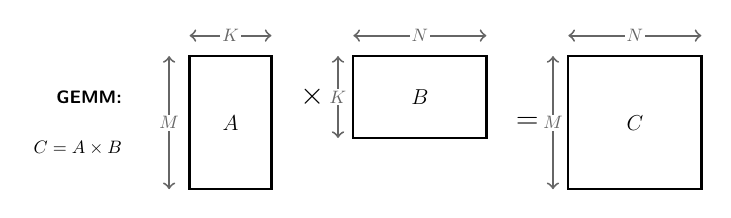
\begin{tikzpicture}[scale=0.65, every node/.style={scale=0.65},
    dim/.style={<->, line width=0.7pt, gray!80!black},
    dlabel/.style={font=\sffamily\bfseries, fill=white, inner sep=1pt}]
  % GEMM label (left side)
  \node[font=\sffamily\bfseries, anchor=east] at (-1.2,1.8) {GEMM:};
  \node[font=\sffamily, anchor=east] at (-1.2,0.8) {$C = A \times B$};

  % --- Matrix A: M rows × K cols ---
  \fill[white] (0,0) rectangle (1.6,2.6);
  \draw[line width=0.8pt] (0,0) rectangle (1.6,2.6);
  \node at (0.8,1.3) {\large $A$};
  % M arrow (left)
  \draw[dim] (-0.4,0) -- (-0.4,2.6) node[midway, dlabel] {$M$};
  % K arrow (top)
  \draw[dim] (0,3.0) -- (1.6,3.0) node[midway, dlabel] {$K$};

  % × sign
  \node at (2.4,1.8) {\LARGE $\times$};

  % --- Matrix B: K rows × N cols ---
  \fill[white] (3.2,1.0) rectangle (5.8,2.6);
  \draw[line width=0.8pt] (3.2,1.0) rectangle (5.8,2.6);
  \node at (4.5,1.8) {\large $B$};
  % K arrow (left)
  \draw[dim] (2.9,1.0) -- (2.9,2.6) node[midway, dlabel] {$K$};
  % N arrow (top)
  \draw[dim] (3.2,3.0) -- (5.8,3.0) node[midway, dlabel] {$N$};

  % = sign
  \node at (6.6,1.3) {\LARGE $=$};

  % --- Matrix C: M rows × N cols ---
  \fill[white] (7.4,0) rectangle (10.0,2.6);
  \draw[line width=0.8pt] (7.4,0) rectangle (10.0,2.6);
  \node at (8.7,1.3) {\large $C$};
  % M arrow (left)
  \draw[dim] (7.1,0) -- (7.1,2.6) node[midway, dlabel] {$M$};
  % N arrow (top)
  \draw[dim] (7.4,3.0) -- (10.0,3.0) node[midway, dlabel] {$N$};

\end{tikzpicture}
\end{center}

\vspace{0.15cm}
\begin{center}
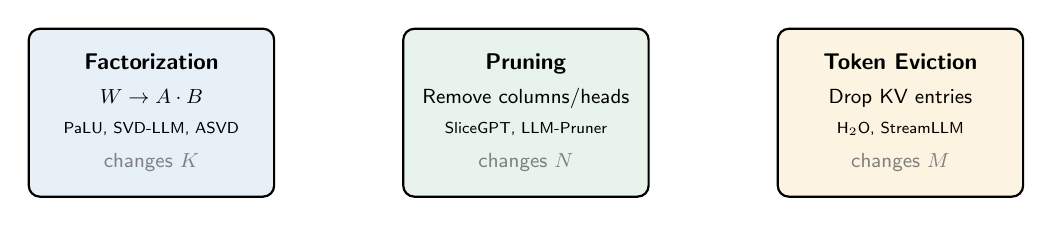
\begin{tikzpicture}[scale=0.82, every node/.style={scale=0.82},
    >=stealth,
    box/.style={draw, rounded corners=4pt, minimum width=3.8cm, minimum height=2.6cm,
                line width=0.8pt, font=\sffamily\small, align=center},
  ]
  % SVD
  \node[box, fill=cblue!12] (svd) at (0,0) {
    \textbf{\normalsize Factorization}\\[4pt]
    $W \to A \cdot B$\\[2pt]
    {\scriptsize PaLU, SVD-LLM, ASVD}\\[4pt]
    \textcolor{gray}{changes $K$}
  };
  % Pruning
  \node[box, fill=cgreen!12] (prune) at (5.8,0) {
    \textbf{\normalsize Pruning}\\[4pt]
    Remove columns/heads\\[2pt]
    {\scriptsize SliceGPT, LLM-Pruner}\\[4pt]
    \textcolor{gray}{changes $N$}
  };
  % Token eviction
  \node[box, fill=corange!12] (token) at (11.6,0) {
    \textbf{\normalsize Token Eviction}\\[4pt]
    Drop KV entries\\[2pt]
    {\scriptsize H$_2$O, StreamLLM}\\[4pt]
    \textcolor{gray}{changes $M$}
  };
\end{tikzpicture}
\end{center}

\vspace{-0.15cm}
\small
Each compression type alters a different GEMM dimension.\\ GPU performance is \textbf{nonlinearly sensitive} to these dimensions.

\end{frame}

% ------------------------------------------------------------
\begin{frame}{The Paradox: Compression Makes Things Slower}
\vspace{-0.1cm}
\begin{columns}
\begin{column}{0.5\textwidth}
\centering
\textbf{Motivating Example}\\[0.2cm]
\small
\begin{tabular}{lccc}
\toprule
& $d$=107 & $d$=112 & \textbf{Penalty} \\
\midrule
GEMM & 0.089\,ms & 0.050\,ms & \textcolor{cred}{\textbf{+78\%}} \\
SDPA & 2.14\,ms & 1.53\,ms & \textcolor{cred}{\textbf{+40\%}} \\
\bottomrule
\end{tabular}

\vspace{0.3cm}
\normalsize
$107 \bmod 8 \neq 0$\\[0.1cm]
$\Rightarrow$ Inefficient PyTorch backend.\\
$\Rightarrow$ Inefficient CUDA kernel\\
$\Rightarrow$ Low-utilization of GPU
\end{column}
\begin{column}{0.5\textwidth}
\centering
\includegraphics[width=0.9\textwidth]{figures/fig3_palu_dist.pdf}

\vspace{0.1cm}
\small
A real example: PaLU on Llama-3-8B, compress 20\% \\
\textbf{78\% layers are misaligned}.
\end{column}
\end{columns}

\vspace{0.2cm}
We call this \textbf{Dimensional Collapse}.
\end{frame}

% ------------------------------------------------------------
\begin{frame}{Budget Allocation: How Are Dimensions Decided?}

\textbf{Current practice}: Given a compression ratio $\rho$, allocate budget based on importance score.

\vspace{0.2cm}
Each method uses a different \textbf{importance score} to allocate per-layer rank $r_i$:

\vspace{0.2cm}
\begin{table}
\centering
\small
\begin{tabular}{@{}llll@{}}
\toprule
\textbf{Method} & \textbf{Score} & \textbf{Intuition} & \textbf{Works} \\
\midrule
Magnitude & $\|W_i\|_F$ & Weight norm & SVD-LLM \\
Activation & $\|X_i\|_F$ & Input magnitude & ASVD \\
Gradient & $\left|\frac{\partial \mathcal{L}}{\partial h_i} \cdot h_i\right|$ & Taylor expansion & Taylor Pruning \\
Fisher & $\mathrm{tr}(\mathbf{F}_i)$ & Curvature of loss & PaLU, FWSVD \\
\bottomrule
\end{tabular}
\end{table}

\vspace{0.2cm}
Scores are \textbf{continuous-valued} $\Rightarrow$ allocated ranks are naturally \textbf{irregular}.
\end{frame}

% ------------------------------------------------------------
\begin{frame}{Misalignment Is Universal Across All Methods}
\begin{center}
\includegraphics[width=0.85\textwidth]{figures/scatter_2x2_meta_llama_3_8b_instruct_r0.8.pdf}
\end{center}

\vspace{-0.1cm}
\small
\textbf{Llama-3-8B}, $r$=0.8. \textcolor{cred}{Red} = misaligned ($d \bmod 8 \neq 0$), \textcolor{cgreen}{green} = 8-aligned. \\
All four methods produce \textbf{50--80\% misaligned} dimensions $\Rightarrow$ structural problem, not edge case.
\end{frame}


% ============================================================
\section{Full-Stack Analysis}
% ============================================================

\begin{frame}{Analysis Overview: Full Stack}
\begin{center}
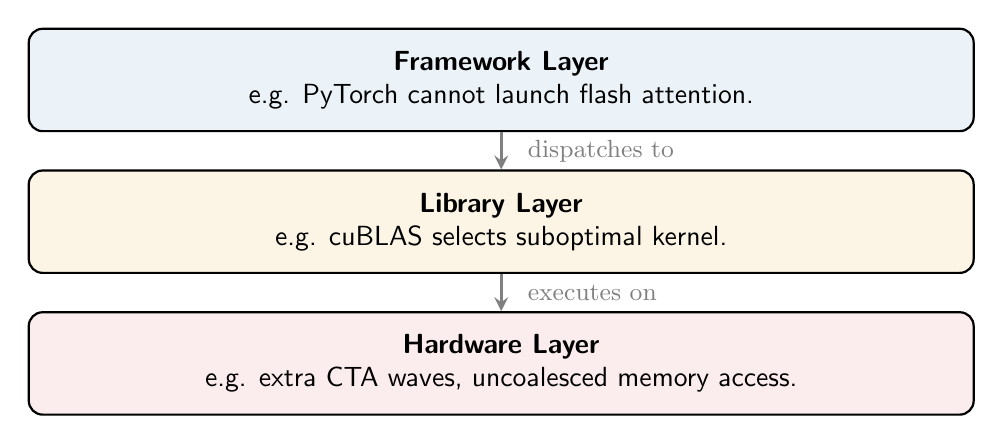
\begin{tikzpicture}[
    layer/.style={draw, rounded corners=5pt, minimum width=12cm, minimum height=1.3cm,
                  line width=0.8pt, font=\sffamily, align=center},
    >=stealth
  ]
  \node[layer, fill=cred!10] (hw) at (0,0) {
    \textbf{Hardware Layer}\\ e.g. extra CTA waves, uncoalesced memory access.
  };
  \node[layer, fill=corange!10] (lib) at (0,1.8) {
    \textbf{Library Layer}\\ e.g. cuBLAS selects suboptimal kernel.
  };
  \node[layer, fill=cblue!10] (fw) at (0,3.6) {
    \textbf{Framework Layer}\\ e.g. PyTorch cannot launch flash attention.
  };

  \draw[->, line width=1.2pt, gray] (fw.south) -- (lib.north) node[midway, right=0.2cm, font=\small] {dispatches to};
  \draw[->, line width=1.2pt, gray] (lib.south) -- (hw.north) node[midway, right=0.2cm, font=\small] {executes on};
\end{tikzpicture}
\end{center}
\end{frame}

% ------------------------------------------------------------
\begin{frame}{Framework Layer: PyTorch SDPA Backend Selection}
\vspace{-0.2cm}
\small
\textbf{Experiment}: Profile PyTorch SDPA function with head dimension $d$=64--256 on A100.

\vspace{-0.1cm}
\begin{columns}[T]
\begin{column}{0.52\textwidth}
\includegraphics[width=\textwidth]{figures/fig2_sdpa_latency.pdf}
\end{column}
\begin{column}{0.46\textwidth}
\small
\textbf{Findings}:
\begin{itemize}\setlength\itemsep{4pt}
\item $d \bmod 8 = 0$: calls \textbf{FlashAttention-2}, otherwise falls back to \textbf{Math backend}
\item $d \bmod 32 = 0$: Perfectly aligned with FA2 template, e.g. less branching and padding overhead.\\
\end{itemize}
\end{column}
\end{columns}
\end{frame}

% ------------------------------------------------------------
\begin{frame}{Library Layer: GEMM Alignment Sensitivity}
\vspace{-0.2cm}
\small
\textbf{Experiment}: Profile cuBLAS \texttt{fp16} GEMM, sweep each dimension ($M$, $N$, $K$) individually on A100.

\vspace{-0.1cm}
\begin{center}
\includegraphics[width=\textwidth]{figures/fig_gemm_alignment.pdf}
\end{center}

\vspace{-0.3cm}
\small
\textbf{Findings}:
\begin{itemize}\setlength\itemsep{2pt}
\item \textbf{Alignment}: $N$ and $K$ show clear \textbf{mod-8 penalty}.
\item \textbf{Cliff}: $M$ and $N$ have \textbf{performance cliffs} where cuBLAS switches CTA tile size.
\end{itemize}
\end{frame}

% ------------------------------------------------------------
\begin{frame}{Library Layer: Why? cuBLAS Kernel Tier System}
\vspace{-0.1cm}
\small
\textbf{Experiment}: Profile cuBLAS kernel selection with Nsight Compute on A100.

\vspace{0.1cm}
\begin{table}
\centering
\small
\begin{tabular}{llll}
\toprule
\textbf{Tier} & \textbf{Condition} & \textbf{Kernel} & \textbf{MMA Instruction} \\
\midrule
\rowcolor{cgreen!10} 1 & dim \% 8 = 0 & cuBLAS-native sm80 & \texttt{mma.m16n8k16} \\
\rowcolor{corange!10} 2 & dim \% 2 = 0 & CUTLASS sm80 align2 & \texttt{mma.m16n8k16} \\
\rowcolor{cred!10} 3 & odd & CUTLASS sm75 align1 & \texttt{mma.m16n8k8} \\
\bottomrule
\end{tabular}
\end{table}

\vspace{0.1cm}
\textbf{Reasons}:
\begin{itemize}\setlength\itemsep{2pt}
\item \textbf{Alignment}: $K$/$N$ alignment determines kernel tier; lower tier $\Rightarrow$ weaker MMA instruction + scalar loads. $M$ is row dimension, not affected by alignment.
\item \textbf{Cliff}: cuBLAS heuristic selects CTA tile size, but switches at non-obvious boundaries (e.g., $M$=1728$\to$1729), causing sudden latency jumps.
\end{itemize}
\end{frame}

% ------------------------------------------------------------
\begin{frame}{Hardware Layer: Why Misalignment Hurts (Working)}
\vspace{-0.1cm}

\begin{itemize}\setlength\itemsep{6pt}
\item \textbf{Tensor Core} --- \texttt{mma.m16n8k16}.\\
  Misaligned forces fallback from \texttt{HMMA} to \texttt{FFMA} (scalar FP math).

\item \textbf{Vectorized Loads} --- \texttt{LDG.128} requires $\text{dim} \bmod 8 = 0$\\
  Misaligned dim falls back to scalar \texttt{LDG.32}, 4$\times$ fewer bytes per instruction.

\item \textbf{L2 Cache Sectors} --- 32-byte fetch granularity\\
  Non-aligned row stride wastes partial sectors, but GEMM tiling largely masks this.
\end{itemize}

\vspace{0.3cm}
\textbf{Takeaway}: The first two mechanisms explain \emph{why} cuBLAS kernel tiers and SDPA backend fallbacks exist at the library/framework level.
\end{frame}

% ------------------------------------------------------------
\begin{frame}{Constraint Summary}
\begin{table}
\centering
\small
\begin{tabular}{@{}lll@{}}
\toprule
\textbf{Layer} & \textbf{Finding} & \textbf{Constraint} \\
\midrule
\rowcolor{cblue!8} Framework & SDPA backend selection & $d \bmod 8 = 0$ \\
\rowcolor{cblue!8} Framework & FA2 template alignment & $d \bmod 32 = 0$ \\
\midrule
\rowcolor{corange!8} Library & cuBLAS kernel tier & $K$/$N$ $\bmod$ 8 = 0 \\
\rowcolor{corange!8} Library & Kernel cliff & heuristics of sweet spot \\
\midrule
\rowcolor{cred!8} Hardware & Tensor Core & $m16n8k16$ \\
\rowcolor{cred!8} Hardware & Vectorized loads & dim $\bmod$ 8 = 0 \\
\rowcolor{cred!8} Hardware & L2 cache sector & dim $\bmod$ 16 = 0 \\
\bottomrule
\end{tabular}
\end{table}

\vspace{0.3cm}
\end{frame}


% ============================================================
\section{GAC: GPU-Aligned Compression \\ The New Compression Paradigm}
% ============================================================

\begin{frame}{GAC Framework Overview}
\vspace{0.3cm}
\begin{center}
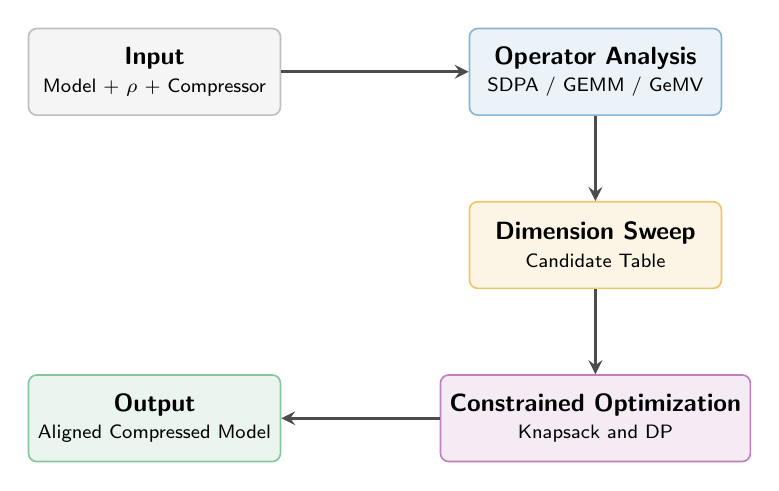
\begin{tikzpicture}[
    >=stealth,
    box/.style={draw, rounded corners=3pt, minimum width=3.2cm, minimum height=1.1cm,
                line width=0.6pt, font=\sffamily\small, align=center},
    arr/.style={->, line width=1.2pt, color=gray!60!black},
  ]

  %% Left column: Input / Output
  \node[box, fill=gray!8, draw=gray!50] (input) at (0, 0)
    {\textbf{Input}\\[-1pt]{\scriptsize Model + $\rho$ + Compressor}};
  \node[box, fill=cgreen!10, draw=cgreen!60] (output) at (0, -4.4)
    {\textbf{Output}\\[-1pt]{\scriptsize Aligned Compressed Model}};

  %% Right column: 3 steps
  \node[box, fill=cblue!10, draw=cblue!60] (ident) at (5.6, 0)
    {\textbf{Operator Analysis}\\[-1pt]{\scriptsize SDPA / GEMM / GeMV}};
  \node[box, fill=corange!10, draw=corange!60] (sweep) at (5.6, -2.2)
    {\textbf{Dimension Sweep}\\[-1pt]{\scriptsize Candidate Table}};
  \node[box, fill=violet!8, draw=violet!50] (opt) at (5.6, -4.4)
    {\textbf{Constrained Optimization}\\[-1pt]{\scriptsize Knapsack and DP}};

  %% Arrows
  \draw[arr] (input)  -- (ident);
  \draw[arr] (ident)  -- (sweep);
  \draw[arr] (sweep)  -- (opt);
  \draw[arr] (opt)    -- (output);

\end{tikzpicture}
\end{center}
\end{frame}

% ------------------------------------------------------------
\begin{frame}{Constrained Optimization (1/3) --- Problem Setup}

\textbf{Setting}: 64 weight matrices in Llama-3-8B, $\rho$=0.7, total budget $B$=46k parameters.

\vspace{0.3cm}
\textbf{Step 1.} Apply existing compressor (e.g. PaLU) $\;\Rightarrow\;$ ideal ranks and Fisher scores:

\vspace{0.2cm}
\centering
\begin{tabular}{@{}lcc@{}}
\toprule
Projection & $r_i^*$ (ideal rank) & $f_i$ (Fisher score) \\
\midrule
$W_1$ (layer 3, k\_proj) & 121.2 & 10.0 \quad {\scriptsize $\leftarrow$ sensitive} \\
$W_2$ (layer 18, v\_proj) & 89.6 & 0.5 \quad {\scriptsize $\leftarrow$ insensitive} \\
$W_3$ (layer 7, k\_proj) & 107.3 & 3.0 \quad {\scriptsize $\leftarrow$ medium} \\
\multicolumn{3}{@{}c@{}}{\footnotesize $\vdots$ \quad (64 projections total)} \\
\bottomrule
\end{tabular}
\raggedright

\vspace{0.4cm}
\textbf{Problem}: These ideal ranks are \textbf{fractional} (121.2, 89.6, 107.3, \ldots).\\
PaLU truncates to integers $\Rightarrow$ \textcolor{cred}{107 hits every GPU cliff we found.}\\[0.2cm]
\textbf{How to round them to hardware-friendly values?}
\end{frame}

% ------------------------------------------------------------
\begin{frame}{Constrained Optimization (2/3) --- Candidate Generation}

\textbf{Step 2.} Dim Sweep near each $r_i^*$ $\;\Rightarrow\;$ keep only \textbf{good} dimensions:

\vspace{0.3cm}
\centering
\begin{tabular}{@{}lcl@{}}
\toprule
Projection & $r_i^*$ & Candidates $C_i$ (low-latency dims from Dim Sweep) \\
\midrule
$W_1$ ($f$=10.0) & 121.2 & \{112, 120, 128\} \\
$W_2$ ($f$=0.5) & 89.6 & \{80, 88, 96\} \\
$W_3$ ($f$=3.0) & 107.3 & \{96, 104, 112, 128\} \quad {\scriptsize 107 excluded --- cliff!} \\
\bottomrule
\end{tabular}
\raggedright

\vspace{0.4cm}
\textbf{Key}: Candidates are \textbf{data-driven} from profiling, not hard-coded \texttt{mod 8}.
\begin{itemize}\setlength\itemsep{0.15em}
\item On A100: cliffs at SDPA template boundaries, cuBLAS kernel tiers
\item On H100: cliffs may shift (TMA 128B, FA3 templates) --- sweep is hardware specific
\end{itemize}
\end{frame}

% ------------------------------------------------------------
\begin{frame}{Constrained Optimization (3/3) --- Knapsack DP}

\textbf{Step 3.} Pick one candidate per projection --- \textbf{maximize total value}:
\[
\max_{\{r_i\}} \sum_{i=1}^{n} \underbrace{f_i \cdot (r_i - r_i^*)}_{\text{value}_i} \quad\text{s.t.}\;\; \sum_{i} \text{params}(r_i) \leq B,\;\; r_i \in C_i
\]

\vspace{0.1cm}
\centering\small
\begin{tabular}{@{}lcccc@{}}
\toprule
 & $r_i^*$ & DP picks $r_i$ & Direction & Value $= f_i \times (r_i - r_i^*)$ \\
\midrule
$W_1$ ($f$=10) & 121.2 & \textbf{128} & $\uparrow$ round up & $10 \times 6.8 = $ \textcolor{cgreen}{\textbf{+68}} \\
$W_2$ ($f$=0.5) & 89.6 & \textbf{88} & $\downarrow$ round down & $0.5 \times (-1.6) = $ \textcolor{cred}{--0.8} \\
$W_3$ ($f$=3) & 107.3 & \textbf{104} & $\downarrow$ slight down & $3 \times (-3.3) = $ \textcolor{cred}{--9.9} \\
\bottomrule
\end{tabular}
\raggedright

\vspace{0.3cm}
$W_2, W_3$ round down, saving budget $\;\Rightarrow\;$ funds $W_1$'s round up.\\[0.1cm]
\textbf{Sensitive layers preserve information; insensitive layers absorb the cost.}\\[0.2cm]
{\footnotesize Multi-choice knapsack DP: $O(n \cdot |C| \cdot B')$, where $B'$ = quantized budget size.}
\end{frame}



% ============================================================
\section{Preliminary Results (Not Yet)}
% ============================================================

\begin{frame}{Planned Experiment:}

\textbf{Setup}: Llama-3-8B, $\rho \in [50\%, 90\%]$.

\vspace{0.3cm}
\textbf{Strategies to compare}:
\begin{itemize}\setlength\itemsep{0.15em}
\item \textbf{Unaligned}: PaLU default --- truncate ideal rank to integer
\item \textbf{Round-to-32}: Independent rounding to nearest multiple of 32
\item \textbf{GAC}: Multi-choice Knapsack + DP
\end{itemize}

\vspace{0.3cm}
\textbf{Metrics}:
\begin{itemize}\setlength\itemsep{0.15em}
\item \textbf{Alignment}: Alignment rate of compressed dimensions
\item \textbf{Accuracy}: PPL on WikiText-2 \& Zero Shot Accuracy
\item \textbf{Latency}: E2E latency (prefill + decode)
\end{itemize}

\vspace{0.3cm}
\textbf{Expect GAC}: 100\% alignment + faster inference  + preserving accuracy.
\end{frame}


% ============================================================
\section{Our Position}
% ============================================================

\begin{frame}{Our Position}

\textbf{1. Mainstream compression is hardware-agnostic.}\\[0.05cm]
{\footnotesize SVD-LLM, FWSVD, ASVD, PaLU, GPTQ, AWQ, \ldots}\\[0.05cm]
Targeting reducing memory, but compressed LLMs are \textbf{dimensionally collapsed}.

\vspace{0.2cm}
\textbf{2. Existing hardware-aware approaches fall short.}\\[0.05cm]
{\footnotesize HALP [Li+ NeurIPS'22], HALOC [Xiao+ AAAI'23]}\\[0.05cm]
Tied to specific compression/model.\\
No guarantee on compression ratio.\\
Does not understand the hardware root-cause.

\vspace{0.2cm}
\textbf{3. Compilers can only react, not prevent.}\\[0.05cm]
{\footnotesize TensorRT / vLLM / TVM}\\[0.05cm]
Pad \emph{up} to the next safe size, wasting memory. \textbf{Cannot change model architecture}.

\vspace{0.2cm}
\hrule
\vspace{0.15cm}
{\small $\Rightarrow$ \textbf{GAC}: A new compression paradigm that wraps any compressor, guarantees parameter budget, and prevents misalignment \textbf{at compression time} via dimension-level root-cause analysis.}
\end{frame}


% ============================================================
\section{Next Steps}
% ============================================================

\begin{frame}{Next Steps}

\textbf{Deadline: 3pm 25/Feb 2026, Saudi Time}

\vspace{0.3cm}
\begin{tabular}{@{}lll@{}}
\toprule
\textbf{Week} & \textbf{Who} & \textbf{Task} \\
\midrule
Feb 4--14 & Jihao & Finish paper writing \\
Feb 15--21 & Tian & Extend experiments to H100 + update paper \\
Feb 22--25 & Jihao & Finalize \& submit \\
\bottomrule
\end{tabular}
\vspace{0.3cm}

\textbf{The Workshop Contributions}:
\begin{itemize}\setlength\itemsep{0.1em}
\item Observe the mismatch between LLM compression and GPU hardware.
\item Quantitative measurement and full-stack root-cause analysis.
\item Propose a new compression paradigm: GAC.
\item Preliminary operator-level experiments with real-LLM shapes.
\end{itemize}
\vspace{0.3cm}
\textbf{We need H100}:
\begin{itemize}\setlength\itemsep{0.1em}
\item Extend current experiments for generalization.
\item TMA 128B hard alignment --- A100's L2 miss was small (H2: 5.8\%), but TMA is a \textbf{hard constraint}.
\item FP8 Tensor Core alignment (m16n8k32)
\end{itemize}
\end{frame}

\end{document}
